% Diagrama TikZ: Comparación visual LPWAN para Smart Energy
% v2: barras escala log, sin gridlines, color por calidad, columna HaLow resaltada

\begin{figure}[ht]
\centering
\resizebox{0.95\textwidth}{!}{%
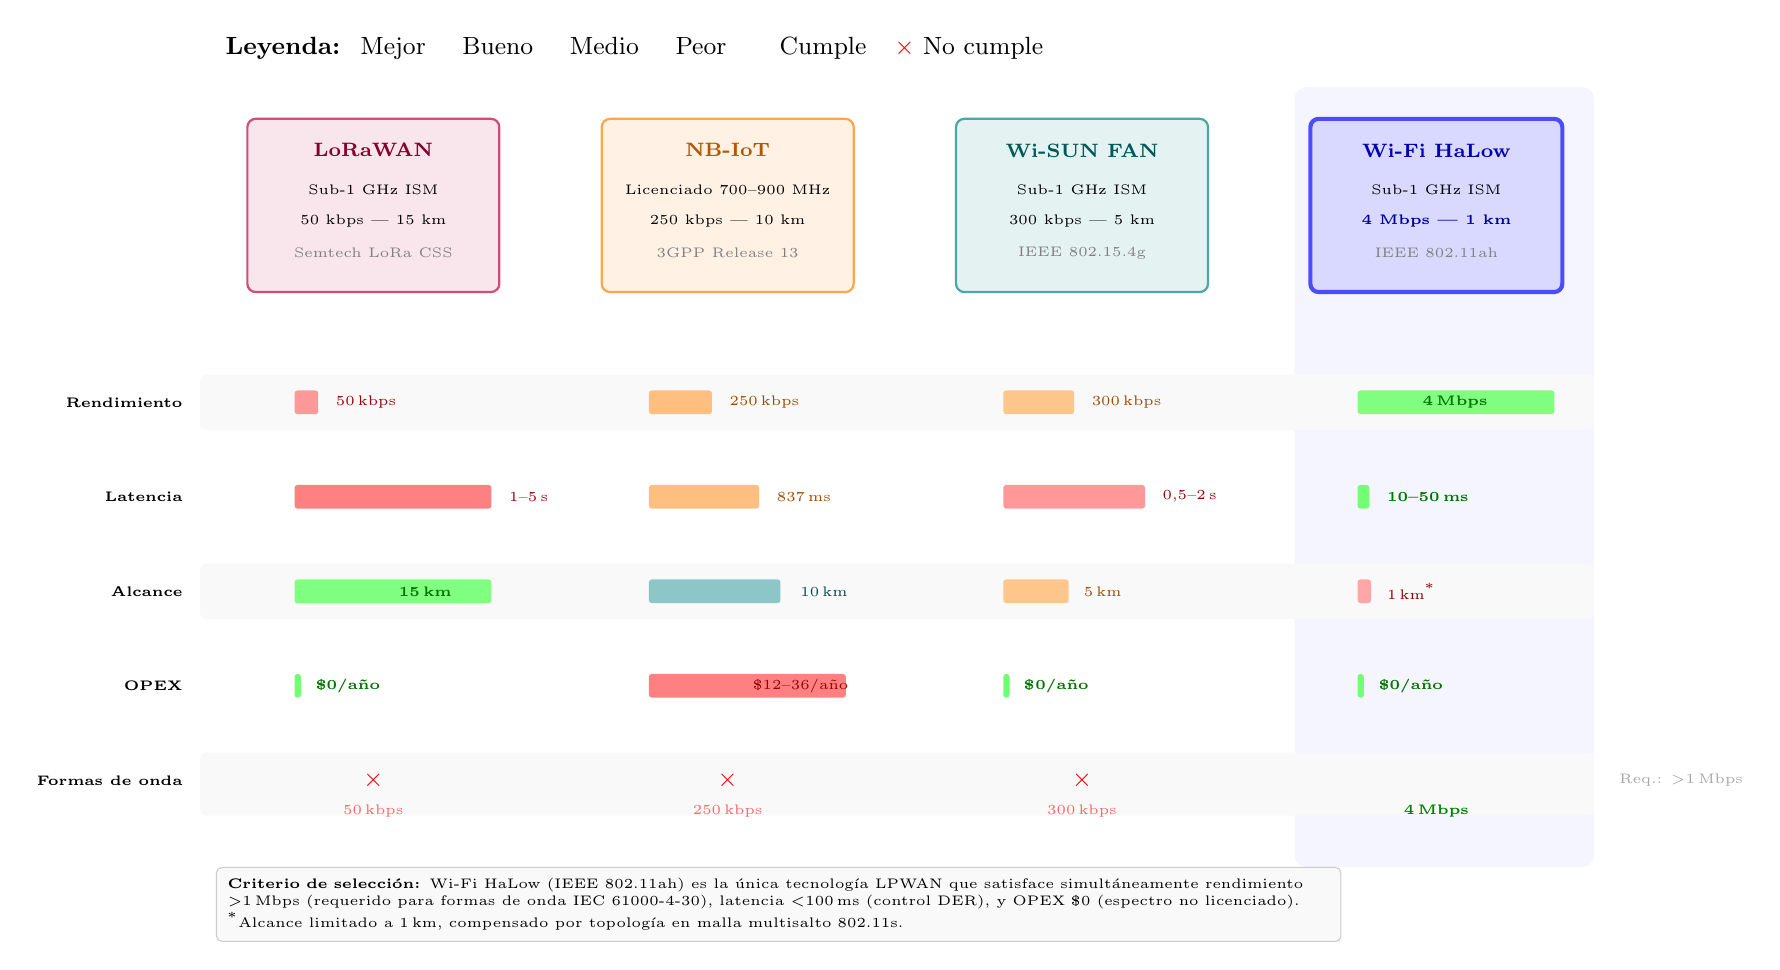
\begin{tikzpicture}[
  techboxbase/.style={rounded corners=3pt, minimum width=3.2cm,
    minimum height=2.2cm, inner sep=4pt, line width=0.8pt, font=\tiny},
  techbox-purple/.style={techboxbase, draw=purple!70, fill=purple!10},
  techbox-orange/.style={techboxbase, draw=orange!70, fill=orange!10},
  techbox-teal/.style={techboxbase, draw=teal!70, fill=teal!10},
  techbox-blue/.style={techboxbase, draw=blue!70, fill=blue!10},
  metric/.style={font=\tiny, #1},
]

% === Leyenda compacta ===
\node[font=\small, anchor=west] at (-2, 2.0) {%
  \textbf{Leyenda:}
  \textcolor{green!55!black}{\footnotesize$\blacksquare$}~Mejor
  \hspace{4pt}
  \textcolor{teal!60}{\footnotesize$\blacksquare$}~Bueno
  \hspace{4pt}
  \textcolor{orange!70}{\footnotesize$\blacksquare$}~Medio
  \hspace{4pt}
  \textcolor{red!60}{\footnotesize$\blacksquare$}~Peor
  \hspace{10pt}
  {\small\textcolor{green!50!black}{\checkmark}}~Cumple
  \hspace{4pt}
  {\small\textcolor{red}{$\times$}}~No cumple
};

% === Resaltado columna HaLow (fondo sutil) ===
\fill[blue!4, rounded corners=4pt] (11.7, -8.4) rectangle (15.5, 1.5);

% === 4 Technology boxes ===

% LoRaWAN
\node[techbox-purple] (lora) at (0, 0) {};
\node[font=\scriptsize\bfseries, purple!70!black] at (0, 0.7) {LoRaWAN};
\node[font=\tiny] at (0, 0.2) {Sub-1 GHz ISM};
\node[font=\tiny] at (0, -0.2) {50 kbps | 15 km};
\node[font=\tiny, gray] at (0, -0.6) {Semtech LoRa CSS};

% NB-IoT
\node[techbox-orange] (nbiot) at (4.5, 0) {};
\node[font=\scriptsize\bfseries, orange!70!black] at (4.5, 0.7) {NB-IoT};
\node[font=\tiny] at (4.5, 0.2) {Licenciado 700--900 MHz};
\node[font=\tiny] at (4.5, -0.2) {250 kbps | 10 km};
\node[font=\tiny, gray] at (4.5, -0.6) {3GPP Release 13};

% Wi-SUN
\node[techbox-teal] (wisun) at (9, 0) {};
\node[font=\scriptsize\bfseries, teal!70!black] at (9, 0.7) {Wi-SUN FAN};
\node[font=\tiny] at (9, 0.2) {Sub-1 GHz ISM};
\node[font=\tiny] at (9, -0.2) {300 kbps | 5 km};
\node[font=\tiny, gray] at (9, -0.6) {IEEE 802.15.4g};

% Wi-Fi HaLow (destacado)
\node[techbox-blue, line width=1.5pt, fill=blue!15] (halow) at (13.5, 0) {};
\node[font=\scriptsize\bfseries, blue!70!black] at (13.5, 0.7) {Wi-Fi HaLow};
\node[font=\tiny] at (13.5, 0.2) {Sub-1 GHz ISM};
\node[font=\tiny\bfseries, blue!60!black] at (13.5, -0.2) {4 Mbps | 1 km};
\node[font=\tiny, gray] at (13.5, -0.6) {IEEE 802.11ah};

% === Barras comparativas (5 métricas) ===
% Escala log-visual para throughput/latencia; lineal para alcance; binaria para OPEX
% Color por calidad: verde=mejor, teal=bueno, orange=medio, red=peor

% ── Fila 1: Rendimiento (mayor = mejor) ──
\def\ry{-2.5}
% Fondo alterno
\fill[gray!5, rounded corners=2pt] (-2.2, \ry-0.35) rectangle (15.5, \ry+0.35);
\node[font=\tiny\bfseries, anchor=east] at (-2.3, \ry) {Rendimiento};
% LoRa 50k (peor)
\fill[red!40, rounded corners=1pt] (-1.0, \ry-0.15) rectangle (-1.0+0.30, \ry+0.15);
\node[metric=red!60!black, anchor=west] at (-0.6, \ry) {50\,kbps};
% NB-IoT 250k
\fill[orange!50, rounded corners=1pt] (3.5, \ry-0.15) rectangle (3.5+0.80, \ry+0.15);
\node[metric=orange!60!black, anchor=west] at (4.4, \ry) {250\,kbps};
% Wi-SUN 300k
\fill[orange!45, rounded corners=1pt] (8.0, \ry-0.15) rectangle (8.0+0.90, \ry+0.15);
\node[metric=orange!60!black, anchor=west] at (9.0, \ry) {300\,kbps};
% HaLow 4M (mejor)
\fill[green!50, rounded corners=1pt] (12.5, \ry-0.15) rectangle (12.5+2.50, \ry+0.15);
\node[metric=green!45!black, anchor=west, font=\tiny\bfseries] at (13.2, \ry) {4\,Mbps};

% ── Fila 2: Latencia (menor = mejor) ──
\def\ly{-3.7}
\node[font=\tiny\bfseries, anchor=east] at (-2.3, \ly) {Latencia};
% LoRa 1-5s (peor)
\fill[red!50, rounded corners=1pt] (-1.0, \ly-0.15) rectangle (-1.0+2.50, \ly+0.15);
\node[metric=red!60!black, anchor=west] at (1.6, \ly) {1--5\,s};
% NB-IoT 837ms
\fill[orange!50, rounded corners=1pt] (3.5, \ly-0.15) rectangle (3.5+1.40, \ly+0.15);
\node[metric=orange!60!black, anchor=west] at (5.0, \ly) {837\,ms};
% Wi-SUN 0.5-2s
\fill[red!40, rounded corners=1pt] (8.0, \ly-0.15) rectangle (8.0+1.80, \ly+0.15);
\node[metric=red!60!black, anchor=west] at (9.9, \ly) {0,5--2\,s};
% HaLow 10-50ms (mejor)
\fill[green!55, rounded corners=1pt] (12.5, \ly-0.15) rectangle (12.5+0.15, \ly+0.15);
\node[metric=green!45!black, anchor=west, font=\tiny\bfseries] at (12.75, \ly) {10--50\,ms};

% ── Fila 3: Alcance (mayor = mejor) ──
\def\ay{-4.9}
\fill[gray!5, rounded corners=2pt] (-2.2, \ay-0.35) rectangle (15.5, \ay+0.35);
\node[font=\tiny\bfseries, anchor=east] at (-2.3, \ay) {Alcance};
% LoRa 15km (mejor)
\fill[green!50, rounded corners=1pt] (-1.0, \ay-0.15) rectangle (-1.0+2.50, \ay+0.15);
\node[metric=green!45!black, anchor=west, font=\tiny\bfseries] at (0.2, \ay) {15\,km};
% NB-IoT 10km
\fill[teal!45, rounded corners=1pt] (3.5, \ay-0.15) rectangle (3.5+1.67, \ay+0.15);
\node[metric=teal!60!black, anchor=west] at (5.3, \ay) {10\,km};
% Wi-SUN 5km
\fill[orange!45, rounded corners=1pt] (8.0, \ay-0.15) rectangle (8.0+0.83, \ay+0.15);
\node[metric=orange!60!black, anchor=west] at (8.9, \ay) {5\,km};
% HaLow 1km (peor, pero compensado por malla)
\fill[red!35, rounded corners=1pt] (12.5, \ay-0.15) rectangle (12.5+0.17, \ay+0.15);
\node[metric=red!55!black, anchor=west] at (12.75, \ay) {1\,km\rlap{\textsuperscript{*}}};

% ── Fila 4: OPEX (menor = mejor) ──
\def\oy{-6.1}
\node[font=\tiny\bfseries, anchor=east] at (-2.3, \oy) {OPEX};
% LoRa $0 (mejor)
\fill[green!55, rounded corners=1pt] (-1.0, \oy-0.15) rectangle (-1.0+0.08, \oy+0.15);
\node[metric=green!45!black, anchor=west, font=\tiny\bfseries] at (-0.85, \oy) {\$0/a\~{n}o};
% NB-IoT $12-36 (peor)
\fill[red!50, rounded corners=1pt] (3.5, \oy-0.15) rectangle (3.5+2.50, \oy+0.15);
\node[metric=red!60!black, anchor=west] at (4.7, \oy) {\$12--36/a\~{n}o};
% Wi-SUN $0
\fill[green!55, rounded corners=1pt] (8.0, \oy-0.15) rectangle (8.0+0.08, \oy+0.15);
\node[metric=green!45!black, anchor=west, font=\tiny\bfseries] at (8.15, \oy) {\$0/a\~{n}o};
% HaLow $0
\fill[green!55, rounded corners=1pt] (12.5, \oy-0.15) rectangle (12.5+0.08, \oy+0.15);
\node[metric=green!45!black, anchor=west, font=\tiny\bfseries] at (12.65, \oy) {\$0/a\~{n}o};

% ── Fila 5: Formas de onda (>1 Mbps requerido) ──
\def\wy{-7.3}
\fill[gray!5, rounded corners=2pt] (-2.2, \wy-0.45) rectangle (15.5, \wy+0.35);
\node[font=\tiny\bfseries, anchor=east] at (-2.3, \wy) {Formas de onda};
% LoRa: no cumple
\node[font=\small, red] at (0, \wy) {$\times$};
\node[metric=red!60, below=1pt] at (0, \wy-0.15) {50\,kbps};
% NB-IoT: no cumple
\node[font=\small, red] at (4.5, \wy) {$\times$};
\node[metric=red!60, below=1pt] at (4.5, \wy-0.15) {250\,kbps};
% Wi-SUN: no cumple
\node[font=\small, red] at (9, \wy) {$\times$};
\node[metric=red!60, below=1pt] at (9, \wy-0.15) {300\,kbps};
% HaLow: cumple
\node[font=\small, green!50!black] at (13.5, \wy) {\checkmark};
\node[metric=green!50!black, below=1pt, font=\tiny\bfseries] at (13.5, \wy-0.15) {4\,Mbps};
% Requisito
\node[metric=gray!70, anchor=west] at (15.7, \wy) {Req.: $>$1\,Mbps};

% === Nota inferior ===
\node[draw=gray!40, fill=gray!5, rounded corners=2pt, font=\tiny,
  text width=14cm, inner sep=4pt, anchor=north west] at (-2, -8.4) {
  \textbf{Criterio de selecci\'{o}n:} Wi-Fi HaLow (IEEE 802.11ah) es la \'{u}nica tecnolog\'{i}a LPWAN que satisface simult\'{a}neamente rendimiento $>$1\,Mbps (requerido para formas de onda IEC~61000-4-30), latencia $<$100\,ms (control DER), y OPEX~\$0 (espectro no licenciado). \textsuperscript{*}Alcance limitado a 1\,km, compensado por topolog\'{i}a en malla multisalto 802.11s.
};

\end{tikzpicture}%
}% end resizebox
\caption{Comparaci\'{o}n visual de tecnolog\'{i}as LPWAN para infraestructura de medici\'{o}n avanzada (AMI). Cinco m\'{e}tricas clave: rendimiento (\textit{throughput}), latencia (menor = mejor), alcance, costo operativo anual (OPEX), y capacidad de transmisi\'{o}n de formas de onda de calidad de energ\'{i}a ($>$1\,Mbps). Wi-Fi HaLow (IEEE 802.11ah, columna resaltada) es la \'{u}nica tecnolog\'{i}a que satisface simult\'{a}neamente rendimiento de 4\,Mbps, latencia $<$50\,ms y OPEX \$0, a costa de alcance limitado (1\,km vs 15\,km LoRaWAN), compensable mediante malla 802.11s.}
\label{fig:lpwan-comparison}
\end{figure}
